\chapter{Generierung modularer Assets}
Für die Bewertung der Ergebnisse dieser Arbeit werden im nächsten Kapitel Qualitätsmerkmale modularer Assets aufgestellt. Der zweite Teil des Kapitels zeigt exemplarisch, inwiefern diese Kriterien erfüllbar sind.
\section{Anforderungen an modulare Assets}
Modulare Assets müssen für den Einsatz in realen Videospiel-Produktionen verschiedene Eigenschaften erfüllen. Diese werden in diesem Abschnitt erläutert.
\subsection{Visuelle Qualität}\label{vqualitaet}
Ein wichtiger Aspekt bei der Entwicklung von Assets ist ihre visuelle Qualität. Sie müssen den restlichen Ansprüchen des Spiels genügen und zu dessen Ästhetik passen.
\par
Insbesondere bei modularen Assets wird dies zu einem Problem, da diese dazu neigen, Elemente häufig zu wiederholen. Man spricht hier von der sogenannten Kunstermüdung (\textit{Art Fatigue}). Sie führt dazu, dass Spieler sich langweilen und das Gefühl haben, bereits alles gesehen zu haben. \parencite{Burgess}
\par
Weiterhin führt die Repetition modularer Assets schnell zu einer Art Orientierungslosigkeit, bei der Spieler nicht mehr genau bestimmen können, wo sie sich gerade befinden. Grund hierfür ist der Mangel eindeutig identifizierbarer Orientierungspunkte. \parencite{unrealModular}.
\par
Zudem gilt es bei der Konzeption modularer Kits darauf zu achten, dass keine Lücken oder Überlagerungen entstehen, da diese zu grafischen Fehlern führen \parencite{Mader}. Sollte es Teile in einem Kit geben, die Lücken zulassen, muss es passende Gegenstücke geben, die diese wieder schließen können \parencite{Burgess}.
 \begin{figure}[!h]
\centering
  \makebox[\textwidth]{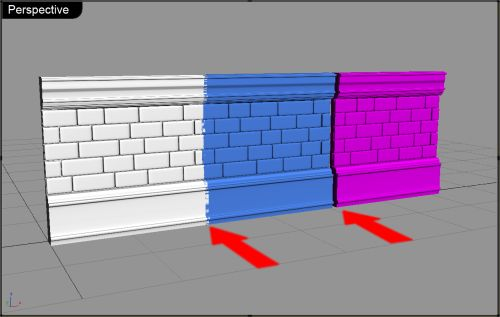
\includegraphics[width=0.7\linewidth]{bilder/glitch}}
  \caption{Beispiel für Überlappung und Lücken zwischen Modulen \parencite{Mader}.}
	\label{glitch}
\end{figure}
\subsection{Nutzerfreundlichkeit}
Damit ein modulares Kit effizient nutzbar ist, muss das Arbeiten mit diesem so angenehm und einfach wie möglich sein. Hierbei ist sehr wichtig, dass sich die einzelnen Teile im Editor einfach bewegen  und verbinden lassen. Nach Möglichkeit sollten diese automatisch einrasten, sobald sie nah genug zusammengeführt werden. \parencite{Mader}.
\par
Auch die Flexibilität trägt erheblich zur Nutzerfreundlichkeit bei. Hierzu zählt, wie kompatibel die einzelnen Teile untereinander sind und wie viel Freiheit sie den Level Designern lassen. \parencite{unrealModular}.
\par
Zusätzlich lässt sich die Nutzerfreundlichkeit daran messen, wie schnell und einfach größere Strukturen erstellt werden können. \parencite{Mader}.
\subsection{Aufwand}
Kosten spielen bei der Erstellung von Videospielen, wie in jeder Branche, eine große Rolle. Um diese möglichst gering zu halten ist es wünschenswert, den benötigten Arbeitsaufwand und die Zeit zu reduzieren. Effektiv entworfene modulare Assets sind hierfür eine gute Hilfe.
\par
In \textit{Skyrim} wurden über 300 Dungeons\footnote{Ein Dungeon ist ein in sich geschlossenes Level, das einen Abschnitt der Spielwelt repräsentiert. Das kann z.B. ein verlassener Tempel, eine Höhle oder ein Verlies sein} von nur zehn Personen entwickelt, darunter nur zwei 3D-Artists. Der Einsatz modularer Assets erlaubte dem Team innerhalb der Entwicklungszeit eine große Menge diverser Spielinhalte zu liefern. \parencite{Burgess}
\par
Ein weiteres Beispiel ist der bereits in Abschnitt \ref{Geschichte von Modularität } erwähnte Einsatz von Modularität in  \textit{For Honor}, bei dem diese genutzt wird, um schnell und einfach Level-Design-Iterationen durchzuführen. \parencite{ForHonor}
\par
Zwar benötigt die Planung modularer Assets vorab mehr Zeit als die Planung herkömmlicher Assets, jedoch ist die Zeitersparnis in der Design-Phase um einiges größer \parencite{Meler}. Ein gutes modulares Asset muss demnach flexibel genug sein, um Level-Design-Iterationen zu beschleunigen.
\subsection{Performance}
Durch das bereits oben erwähnte \textit{Instancing} (vgl. Abschnitt \ref{Implementierung1}) können modulare Assets helfen, die Performance des Spiels zu verbessern und somit eine höhere Bildfrequenz zu erreichen.
\par
Entscheidend hierfür sind die Modularitätsstufen (vgl. Abschnitt \ref{mstufe}) und die Wiederverwertbarkeit der Assets, damit das Instancing effektiv genutzt werden kann.
\newpage
\subsection{Zusammenfassung}
Die Qualität modularer Assets lässt sich über mehrere Kriterien bewerten. Für den weiteren Verlauf der Arbeit sind die genannten Kriterien ein ausschlaggebendes Bewertungsmaß der erstellten Assets. Hier eine Übersicht der aufgestellten Kriterien:
\begin{itemize}
\item Visuelle Qualität: Lücken und Überlappungen sollten vermieden werden. Um die Kunstermüdung zu vermeiden, sollte das Kit über ausreichend Abwechslung oder musterbrechende Teile verfügen. Starke Wiederholungen sollten vermieden werden.
\item Nutzerfreundlichkeit: Ein gutes modulares Kit ermöglicht einfaches Arbeiten. Zusammenfügen und Bewegen der Teile ist einfach und intuitiv. Die Teile erlauben den Bau größerer Strukturen ohne großen Mehraufwand. Das Kit ist untereinander flexibel und kompatibel.
\item Aufwand: Die Assets helfen in der späteren Projektphase Level Design Iterationen zu verkürzen und ermöglichen die Erstellung einer Vielzahl von Inhalten mit möglichst wenigen Assets.
\item Performance: Das modulare Kit kostet nicht mehr Performance, als ein herkömmliches und erzielt bestenfalls durch Instancing eine noch bessere Performance.
\end{itemize}
\newpage
\section{Methoden für die Generierung modularer Assets}
Um die Planung und die Produktion modularer Kits so effektiv wie möglich zu gestalten, sollten bestimmte Regeln und Vorgehensweisen beachtet werden. Im Folgenden werden die wichtigsten davon erläutert.
\subsection{Projektübergreifende Planung}
Planung ist nach Klafke und Meler einer der wichtigste Aspekt bei der Entwicklung modularer Assets \parencite{Klafke,Meler}.
\par
Sie kann in zwei Stufen eingeteilt werden. Während die erste der beiden Phasen nur einmal im Verlauf des gesamten Projektes durchgeführt werden muss\footnote{\,Dies gilt unter der Annahme, dass alle Kits nach den gleichen Regeln erzeugt werden. Andernfalls muss auch die erste Phase für jedes Kit wiederholt werden.}, muss die zweite für jedes neue Kit im Projekt ausgeführt werden. \parencite{Burgess}
\par
In der ersten Planungsphase werden grundlegende Eigenschaften der angestrebten Modularität festgelegt. Hierzu gehören die verwendeten Modularitätsstufen, die Abstimmung einheitlich verwendeter Rasters \parencite{Perry} und das Setzen der Pivot Points \parencite{Mader}. Auf Grund ihrer Bedeutung und Komplexität werden diese im Folgenden detailliert beleuchtet. Sollten alle erstellten Kits diesen gemeinsamen Regeln folgen, sind sie auch untereinander kombinierbar und können somit für mehr Diversität sorgen \parencite{Burgess}.
\subsection{Modularitätsstufen}\label{mstufe}
Entsprechend des Grades ihrer Aufspaltung in Einzelteile teile L. Perry modular angelegte Assets in verschiedene Stufen (im Original \enquote{Scales}) ein \parencite{Perry}.
\par
Die verwendeten Modularitätsstufen sollten zu Beginn der Planung festgelegt werden, damit die folgenden Schritte einfacher konkretisiert werden können \parencite{unrealModular}.  Die gewählte Stufe ist abhängig von der Spielwelt und dem geplanten Grad der Modularität \parencite{unrealModular}. Wurden diese festgelegt, können die benötigten Gebilde leichter in Module unterteilt werden, die der benötigten Stufe entsprechen. Die Ausprägungen der Stufen werden jetzt erläutert.

\begin{figure}[!h]
\centering
  \makebox[\textwidth]{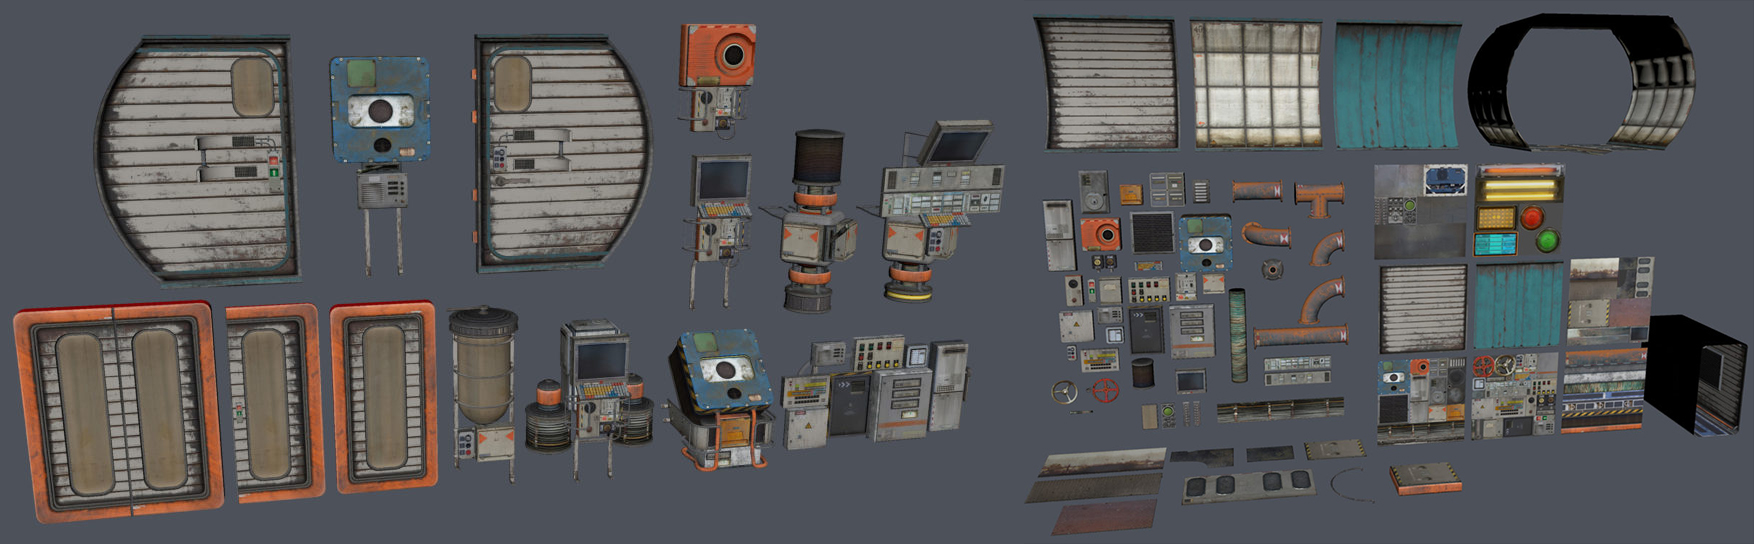
\includegraphics[width=1\linewidth]{bilder/spacemodular}}
  \caption{Module für den Innenraum einer Raumstation. In Anlehnung an \parencite{spacemodular}.}
	\label{spacemodular}
\end{figure}
Für Innenräume empfiehlt sich ein stark granulares Kit, damit Wände, Böden und andere Teile der Umgebung detail- und abwechslungsreich zusammengesetzt werden können. Beispiel für einen solchen Innenraum wäre eine verlassene Raumstation, die nur schleichend erkundet wird \parencite{Perry}.
\par
Abbildung \ref{mittlereStufe} zeigt ein modulares Kit mit mittlerer Modularitätsstufe. Jedes Element aus dem Kit ist eine eigene Wand, mit dessen Hilfe ein Gebäude erstellt werden kann. Eine Mischung aus einer solchen Modularitätsstufe und einer kleineren wurde von  L. Durand für \textit{For Honor} genutzt (vgl. Abbildung \ref{ForHonorImage}).

\begin{figure}[!h]
\label{StufenBilder}
\centering
  \subfloat[][Übersicht eines Kits mit mittlerer Modularität.]{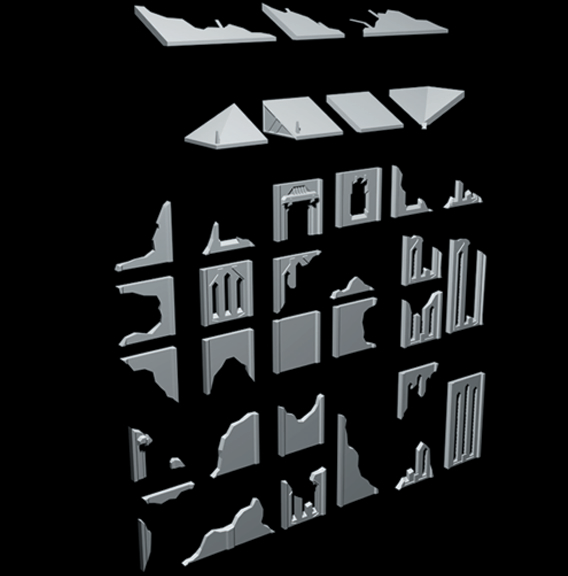
\includegraphics[width=0.45\linewidth]{bilder/ScaleKlein}\label{mittlereStufe}}%
  \qquad
  \subfloat[][Übersicht eines Kits mit geringer Modularität.]{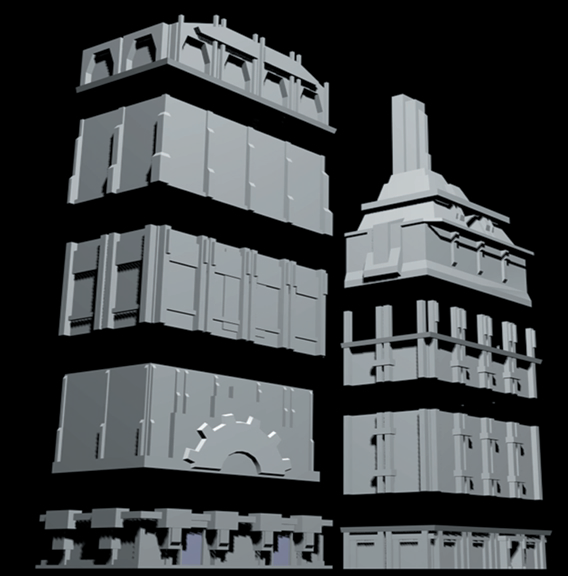
\includegraphics[width=0.45\linewidth]{bilder/ScaleGross}\label{grosseStufe}}%
  \caption{Beispiele für verschiedene Modulraitätsstufen eines Gebäude Kits \parencite{Perry}.}%
\end{figure}
Ein Beispiel für eine geringe Modularitätsstufe zeigt \ref{grosseStufe}. Mit Hilfe dieses Kits können Gebäude aus verschiedenen, vorgefertigten Etagen zusammengesetzt werden. Sie erlauben schnell eine Vielzahl unterschiedlicher Gebäude zu erstellen, jedoch sind diese aufgrund der geringen Modularität recht einseitig.
\par
In der nächstgrößeren Stufe würden ganze Häuser genutzt, um daraus Häuserblöcke zu errichten. Eine weitere Steigerung wäre aus diesen Häuserblöcken eine Stadt zu errichten. Diese Modularitätsstufe eignet sich beispielsweise für den Einsatz in einem Rennspiel. \parencite{Perry}
\par
Innerhalb eines Projekts können durchaus verschiedene Stufen verwendet und gemischt werden. Besitzt ein Spiel beispielsweise offene und geschlossene Bereiche, so ist es sinnvoll, deren Kits für diese unterschiedlich modular zu gestalten. Das gleiche Spiel für Bereiche, die der Spieler aus verschiedenen Distanzen sieht. So könnten bei einem Fußweg durch die Stadt beispielsweise die Häuserreihen weniger modular sein als die Straße, über die der Spieler läuft, da letztere deutlich präsenter und näher ist. \parencite{Klafke}
\par
Beim Arbeiten mit nur einer einzigen Stufe kann die Repetition durch die manuelle Platzierung kleinerer Objekte aufgebrochen werden \parencite{Perry}.
\par
Die Modularitätsstufen sollten zudem projektspezifisch betrachtet werden. Für ein Rennspiel im Weltall, dessen kleinste Einheit Raumschiffe sind, ist es wenig sinnvoll die gleichen Modularitätsstufen zu nutzen wie für ein Fantasy-Rollenspiel mit detailliertem Interieur. Die Einteilung der Stufen ist immer auch abhängig von der Spielwelt und Perspektive.
\enlargethispage{10.5pt}
\subsection{Raster}\label{Rasterkapitel}
Nach L. Durand ist einer der wichtigsten Aspekte, für die Umsetzung eines Projekts mit modularem Design, das Raster \parencite{ForHonor}.
\par
Jedes 3D-Tool arbeitet intern mit einem Raster\footnote{\,Das Raster ist hier ein dreidimensionales Koordinatensystem.}. Sie können sich in der verwendeten Maßeinheit (Meter, Zentimeter, ...), der Orientierung des Koordinatensystems, den Unterteilungsstufen und anderen Eigenschaften unterscheiden. Im Raster ist es 3D-Artists möglich, Objekte punktgenau im Raum zu platzieren. Dies ermöglicht die Erstellung modularer Assets mit lückenlosen Übergängen. \parencite{Mader}
\begin{figure}[!h]
\label{RasterBilder}
\centering
  \subfloat[][Beispielhafte Kalkulation der Raster-Einteilungen.]{\includegraphics[width=0.47\linewidth]{bilder/RasterEinteilung}\label{RasterSizes}}%
  \qquad
  \subfloat[][Beispiel für die Angleichung von Modulen.]{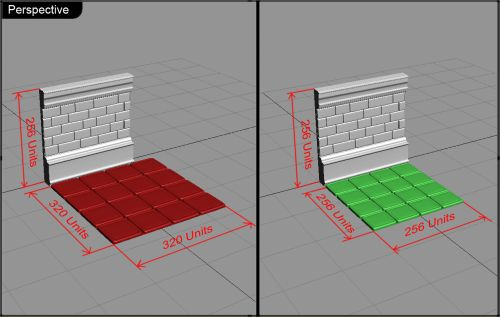
\includegraphics[width=0.47\linewidth]{bilder/GleichGrosseObjekte}\label{sameRasterSize}}%
  \caption{Beispiele für die Anwendung verschiedener Rastergrößen \parencite{Mader}.}%
\end{figure}
Das Raster sollte möglichst in Stufen von Zweierpotenzen eingeteilt sein. Nur durch das Nutzen von geraden Zahlen kann das Raster in kleinere Stufen aufgeteilt werden. Dies kann für kleinere Objekte nötig sein. Kann die Größe eines Elements nicht durch die standardmäßig genutzte Zweierpotenz dargestellt werden, ist es möglich, kleinere Zweierpotenzen zu addieren oder subtrahieren. Abbildung \ref{RasterSizes} zeigt Beispiele für mögliche Einteilungen des Rasters. \parencite{Mader}
\par
Zu kleine Einteilungen des Rasters, erhöhen jedoch den Aufwand des Zusammenbaus von Elementen. Die Module müssen dann in immer kleineren Schritten über das Raster bewegt werden, wodurch das Einrasten erschwert wird. \parencite{Mader} 
\par
Alle Elemente, die untereinander kompatibel sein sollten, wie beispielsweise Wände, Böden und Decken, sollten die gleichen Grundmaße besitzen, da sie ansonsten nur schwer untereinander kombinierbar sind. \parencite{Mader}
\par
Abbildung \ref{sameRasterSize} illustriert dieses Problem: Die Wand und die rote Bodenfläche sind untereinander nicht kompatibel, ohne dass eines der beiden Elemente größer bzw. kleiner skaliert oder fünf Wand- und vier Bodenelemente benutzt werden. Eine solche Inkompatibilität sorgt für erhöhten Zeitaufwand und eine Einschränkung der kreativen Freiheit der Level-Designer. So verliert sich der Mehrwert der angestrebten Modularität.
\par
Burgess und Purkypile bezeichnen die Grundmaße eines Kits als Footprint (deutsch Fußabdruck). Passt ein Element nicht in den definierten Fußabdruck, sollte es entweder ein Vielfaches oder einen Teiler der Größe des Fußabdruck als Größe nutzen \parencite{Burgess}.
\enlargethispage{10.5pt}
\newpage
Beispielsweise könnte die grüne Bodenfläche aus Abbildung \ref{sameRasterSize} auch die Größe 128x128 besitzen. Dann müssten vier Elemente genutzt werden, um die Fläche vor der Wand zu füllen, die gewünschte Modularität bliebe zu einem gewissen Grad erhalten.
 \begin{figure}[!h]
\centering
  \makebox[\textwidth]{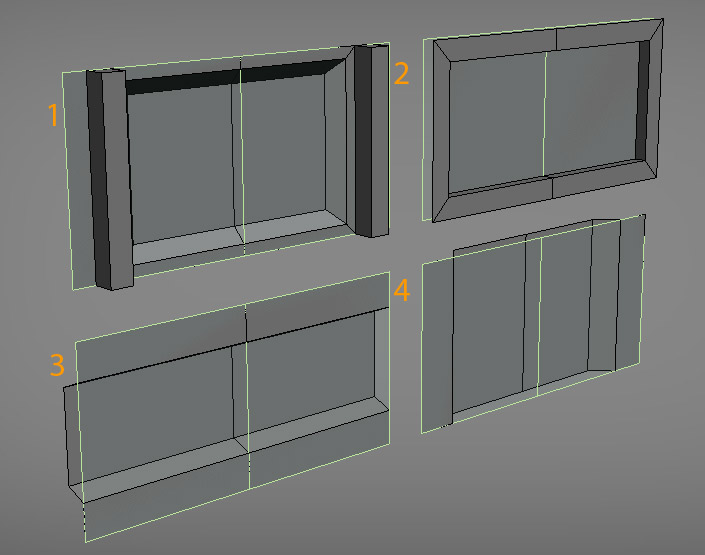
\includegraphics[width=\linewidth]{bilder/boundingBox}}
  \caption{Beispiel für verschiedene Qualitäten von Kontaktpunkte \parencite{Klafke}.}
	\label{boundingBox}
\end{figure}
\par
Thiago Klafke arbeitet mit \textit{Bounding Boxes}. Alle Module in seinem Kit müssen in eine vorgegebene Box passen. Sie muss nicht in alle Richtungen gefüllt sein, aber ihre Kanten sollten nach Möglichkeit soweit ausgearbeitet sein, dass keine Lücken zwischen den Modulen entstehen. Haben Module eine Tiefe, sollten alle Elemente an den Rändern der \textit{Bounding Box} auf der gleichen Ebene liegen. Abbildung \ref{boundingBox} verdeutlicht dies: Werden z.B. die Elemente 1 und 3 horizontal mit einander verbunden entstehen Lücken. Modul 2 ist in diesem Fall weder mit 1 noch mit 3 oder 4 kombinierbar, da es mit keinem dieser Module verbunden werden kann, ohne Lücken zu erzeugen. \parencite{Klafke}
\par
Die Einteilung der Raster-Größe und seiner Aufteilung sollten abhängig von der Größe der Spielfigur, der Animationen und der Bewegung des Spielers in der Welt entschieden werden \parencite{Perry}. Wenn vorhanden, muss auch die Interaktion von Computer gesteuerten Charakteren mit der Umwelt mit einbezogen werden \parencite{Burgess}. \textit{Skyrim} beispielsweise nutzt als minimale Größe eines begehbaren Elements die Breite von zwei Charakteren, wodurch sichergestellt wird, dass sich alle Figuren frei bewegen können \parencite{Burgess}.
\par
Um die Fehleranfälligkeit zu verringern und den Arbeitsprozess zu beschleunigen, sollten die unterschiedlichen Rasters aller verwendeten 3D-Tools aneinander angeglichen werden. Diese Angleichung sollte optimalerweise direkt im Anschluss an die Konzeption des Rasters erfolgen. \parencite{ForHonor}
\enlargethispage{11.5pt}
\par
\subsection{Positionierung und Nutzen des Pivot Points}
Der Pivot Point (Drehpunkt) oder auch der Origin Point (Ursprung) kann beliebig für jedes Objekt gesetzt werden \parencite[S.\,85]{blender}. Über ihn wird definiert, wo sich das Objekt im Raum befindet und wie sich Rotation, Skalierungen und Spiegelungen darauf auswirken \parencite[S.\,85 \& S.102]{blender}.
\par
Ohne korrekt gesetzten Pivot Point wird die zielgenaue Platzierung eines Objektes im dreidimensionalen Raum erschwert bzw. ist nur eingeschränkt möglich. Ein falsch positionierter Pivot Point schränkt die Vorteile der Modularität ein und beeinflusst den Workflow negativ. \parencite{Mader,ForHonor}
\par
Im Folgenden werden verschiedene Beispiele gezeigt, anhand derer Regeln zur korrekten Platzierung des Pivot Points, für jedes Objekt bzw. Objektgruppe, abgeleitet werden können. Sind Objekte auf einer oder mehreren Achsen symmetrisch, sollte der Pivot Point am Ursprung des lokalen Koordinatensystems des Objekts platziert werden. Dadurch kann mit diesem in der Engine freier gearbeitet werden. \parencite{Mader}
\par
Wie zu fast allem gibt es auch zu der Platzierung des Pivot Points einige fallspezifische Ausnahmen. 
\par
Zusätzlich muss beachtet werden, dass eine nachträgliche Änderung des Pivot Points dazu führt, dass jede Instanz des Objektes im Spiel angepasst werden muss, da z.b. eine Translation des Pivot Points auch zu einer Translation des Objektes in der Spielwelt führt. \parencite{Burgess}
\begin{figure}[!h]
\centering
  \makebox[\textwidth]{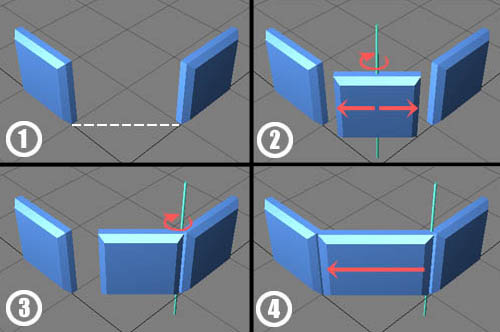
\includegraphics[width=\linewidth]{bilder/cornerPiece}}
  \caption{Beispiel für den Einsatz eines am Ende einer Mauer platzierten Pivot Points \parencite{unrealModular}.}
	\label{cornerPiece}
\end{figure}
\par
Bei Objekten, die entlang einer Achse wiederholt werden sollen, sollte der Pivot Point möglichst an einem der beiden Enden der Achse positioniert werden (Abbildung \ref{cornerPiece}). \parencite{Mader}
\enlargethispage{10.5pt}
\newpage
Für sich wiederholende Objekte sollte der Pivot Point bei allen Objekten der gleichen Art auf der gleichen Seite der entsprechenden Achse liegen, damit eine einfache Verbindbarkeit der Module gewährleistet ist \parencite{Mader}.
\par
Ein weiteres Beispiel, warum es von Vorteil ist, für Mauer- oder Wandstücke den Pivot Point an einer Seite zu haben, ist das Überbrücken einer Lücke mit einem Winkel. Abbildung \ref{cornerPiece} stellt diesen Fall dar. Wäre der Pivot Point in der Mitte des Moduls, wäre das Anpassen an die Größe der Lücke und das Setzen an die richtige Position mit viel Aufwand verbunden. \parencite{Perry}
\par
Bei, auf dem Boden oder einer anderen Fläche platzierten, Elementen, sollte der Pivot Point möglichst an der Unterseite des Objektes positioniert werden, damit diese bei aktivierter Einrastfunktion auch wirklich mit dem Grund der Spielwelt abschließen. Durch diese Technik können spätere händische Eingriffe verhindert werden. Außerdem ändern diese Objekte dadurch auch nicht ihre Position auf dem Boden, wenn sie skaliert werden. \parencite{Mader}
\par
Für Elemente, die unter oder direkt neben anderen platziert werden, sollte der Pivot Point an die Ecke gesetzt werden, die mit den benachbarten Objekten in Kontakt kommen sollen. So kann das Element in genau dieser Ecke einrasten. Ein Beispiel hierfür könnte eine Stuckleiste sein, die zwischen Decke und Wand eingesetzt wird. \parencite{Meler}
\par
Diese Regeln können teilweise auch untereinander kombiniert werden. Soll beispielsweise die Leiste aus dem vorigen Beispiel noch horizontal erweiterbar sein, muss der Pivot Point zusätzlich an einer der äußeren Ecken platziert werden (vgl. Abbildung \ref{stuck}). \parencite{Meler}
\begin{figure}[H]
\centering
  \makebox[\textwidth]{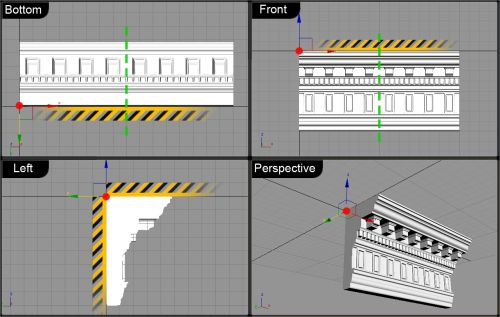
\includegraphics[width=\linewidth]{bilder/stuck}}
  \caption{Beispiel für die Positionierung eines Pivot Points an einer Stuckleiste \parencite{Mader}.}
	\label{stuck}
\end{figure}
\newpage
Eine etwas unintuitive Ausnahme bilden Objekte mit einer Krümmung in ihrer Oberfläche. Für diese empfiehlt es sich, den Pivot Point in das Zentrum des Kreises der Krümmung zu setzen (Abb.\ref{pivotRotation}). Dadurch ist er zwar weit weg vom eigentlichen Objekt, allerdings ergibt sich durch die Krümmung ein nützlicher Vorteil: Wenn die Pivot Points der einzelnen Elemente überlagern, können diese durch simple Anpassung der Rotation sehr leicht aneinander angelegt werden. \parencite{Mader}
\begin{figure}[H]
\centering
  \makebox[\textwidth]{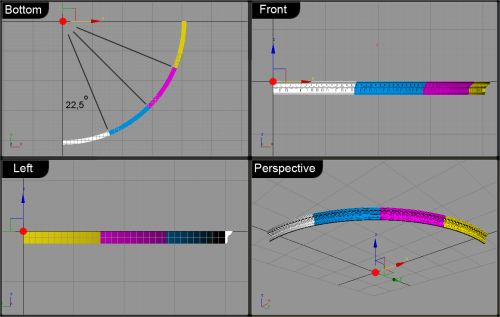
\includegraphics[width=\linewidth]{bilder/pivotRotation}}
  \caption{Beispiel für einen Pivot Point im Zentrum eines Kreises \parencite{Mader}.}
	\label{pivotRotation}
\end{figure}
\vspace{-10.5pt}
\subsection{Kit-spezifische Planung}\label{Kit Spezifische Planung}
In der zweiten Planungsphase werden die Details des Kits ausgearbeitet und spezifische Regeln definiert. Während dieser Phase wird das Setting festgelegt, welches das Kit abbilden soll \parencite{Burgess}. Das können beispielsweise vereiste Höhlen oder das Innere eines Raumschiffs sein. Außerdem sollte geklärt werden, wie und mit welchem Zweck das Kit im Spiel eingesetzt wird, damit sein Umfang und seine Möglichkeiten entsprechend planbar sind \parencite{Burgess}. Nach Perry ist es eine gute Methode dafür eine Liste mit allen Eigenschaften, die das Kit erfüllen soll. Dabei geht es primär um die Kernelemente des Kits, welche für den Großteil des Einsatzgebietes genutzt werden \parencite{Perry}.
\par
Einzigartige Modelle, so genannte \textit{Hero Pieces}, sollten erst im späteren Verlauf entwickelt werden. Sie trügen in der frühen Phase wenig zum Fortschritt des Kits bei, benötigten aber viel Arbeit und ihr Fehlen verzögerte im Gegensatz zu den Kernelementen des Kits nur an wenigen Stellen den Arbeitsablauf. \parencite{Burgess,Perry}
\par
Joel Burgess fordert in einem GDC-Talk zu validieren, welche Kits eine Existenzberechtigung haben.Können Kits zusammengefasst werden, um ein generalisiertes Kit mit vielseitigerem Nutzen zu erzeugen, sei dies empfohlen. Dies verringere die Anzahl und die Planungszeit der benötigten Kits und so auch die Komplexität des Projekts. \parencite{Fallout4}
\par
Perry, Burgess und Purkeypile empfehlen einheitlich, dass Kits Elemente enthalten sollten, mit denen sie untereinander verbunden werden könnten \parencite{Burgess,Perry}. So könne z.B. eine einheitliche Größe für Türrahmen genutzt werden, um den Übergang von einem in das nächste Kit zu schaffen, ohne für beide spezifische Teile anfertigen zu müssen \parencite{Burgess}.
Perry erwähnt zusätzlich, dass Kits abgrenzende Elemente benötigten. So solle für einen modularen Fluss beispielsweise ein Wasserfall oder eine Mündung in ein Gitter existieren, damit der Fluss beendet werden könne \parencite{Perry}. So lange ein Kit nicht für die Generierung endloser Objekte/Level gedacht sei, sei die Einplanung solcher Teile zwingend.
\par
Für das weitere Vorgehen gibt es verschiedene Methoden, bei denen teilweise die Planungsphase in die Erstellungsphase über geht.
\par
Klafke und Norris empfehlen beide, mit der Erstellung von Texturen und Materialien zu beginnen, bevor die ersten Modelle existieren \parencite{Klafke,Norris}. Obwohl sie hier einig sind, unterscheiden sich ihre Vorgehensweisen:
\par
Norris erzeugt für seine Kits bereits voll ausgearbeitete Texturen mit allen Details, die er abbilden möchte, bevor er die Modelle erstellt  \parencite{Norris}. Klafke hingegen arbeitet etwas freier. Für ihn ist ein Mockup der späteren Textur ausreichend, um die Modelle passend zu unwrappen und dadurch im weiteren Verlauf Zeit zu sparen \parencite{Klafke}.
\par
Der Aufbau der genutzten Texturen ist bei beiden ähnlich und besteht aus großen, kachelbaren Texturen, um Wände abzubilden \parencite{Klafke,Norris}. Klafke nutzt diese zusätzlich auch für Bodenflächen \parencite{Klafke}. Für alle im Kit darzustellenden Details erstellen sie eine, beziehungsweise zwei Texturen mit einer Verbindung aus Trims, so genannte Trim Sheets\footnote{\,Trim Sheets sind Texturen, die mehrere unabhängige und meist kachelbare Details enthalten \parencite{Meler}.} \parencite{Klafke,Norris}.
\par
Eine weitere Vorgehensweise wird von Burgess und Purkeypile beschrieben. Hier wird mit der Erstellung einfacher Modelle begonnen, anhand derer alle aufgestellten Regeln und erarbeiteten Ideen ausgiebig getestet werden. Es ist möglich, dass in dieser Phase viele Modelle entstehen, die verworfen werden, bevor eine Herangehensweise gefunden wird, um passende Assets zu erstellen. In dieser Zeit können die Regeln des Kits noch einfach verändert  und auf die Bedürfnisse des Spiels angepasst werden. \parencite{Burgess}
\par
Die nächste Stufe dieses Prozesses ist das sogenannte Grayboxing. In dieser Phase werden die Kernelemente des Kits mit einem geringen Detailgrad und ohne Texturen erstellt. Das Grayboxing dient weiterhin dazu, das Konzept des Kits sowie die Funktionen der einzelnen Module zu überprüfen und solange zu verfeinern, bis alle Elemente auf dem gewünschten Niveau sind. Die visuelle Qualität der Elemente spielt dabei noch keine große Rolle, der Fokus liegt auf der Funktionalität. Können die Elemente des Kits alle Probleme lösen, für die es konzipiert wurde, kann die Phase beendet werden. \parencite{Burgess}
\par
Nach der Graybox-Phase werden alle Assets ausgearbeitet. Aus den vorher entworfenen Elementen werden detailreiche, texturierte Assets erstellt und für die weitere Verarbeitung freigegeben. Zusätzlich werden weniger prominente Teile erstellt, die in der vorherigen Phase ausgelassen wurden. Existieren Varianten von Assets, sollte erst eine Version fertig gestellt werden, um final testen zu können, dass es keine Probleme gibt. So kann vermieden werden, dass alle Varianten überarbeitet werden müssen, wenn es zu Fehlern kommt. Sowohl während dieses Vorgangs als auch danach werden alle Assets verfeinert. Es werden bestehende Fehler und Unreinheiten ausgebessert und die Kits, falls nötig, um Module erweitert, bis das Projekt beendet ist. \parencite{Burgess}
\par
Eine dritte Vorgehensweise wird von Perry angeführt. Ihm zufolge sollten erst einfache modulare Modelle erstellt und dann nach und nach weitere komplexere Teile hinzugefügt werden. Unterstützend zu dieser Arbeit soll eine Asset-Review eingeführt werden, bei der regelmäßig getestet wird, ob alle bisher produzierten Modelle wie vorgesehen untereinander kompatibel sind und funktionieren. Dies soll gewährleisten, dass am Ende keine fertigen Assets erzeugt werden, die nicht ohne aufwändige Überarbeitungen funktionieren. \parencite{Perry}
\par
Ein bisher unerwähnter Aspekt ist die Namensgebung der modularen Assets. Bereits früh im Projekt sollte eine passende Namenskonvention eingeführt werden, die auf alle Kits anwendbar ist. Dies sorgt dafür, dass alle Artists, Designer und Programmierer immer genau wissen, welchen Zweck ein bestimmtes Modul hat und damit schneller und effizienter arbeiten können. \parencite{Burgess}

\begin{figure}[!h]
\centering
  \makebox[\textwidth]{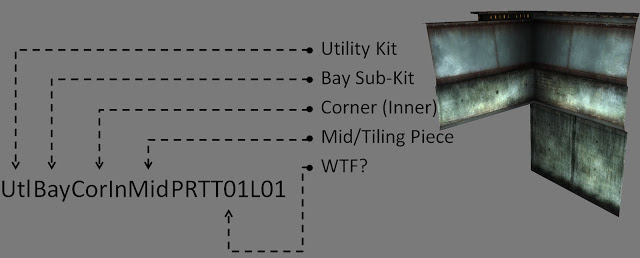
\includegraphics[width=\textwidth]{bilder/namingConvention}}
  \caption{Beispiel für Namensgebung eines modularen Assets aus \textit{Fallout 3} \parencite{Burgess}.}
	\label{namingConvention}
\end{figure}
Abbildung \ref{namingConvention} zeigt beispielhaft die Kodierung einer sinnvollen Namenskonvention. Der Name sollte möglichst deskriptiv und einfach zu entschlüsseln sein. Zudem ist es sinnvoll, eine bei \enquote{01} beginnende und aufsteigende Nummerierung einzuführen. Dies erleichtert die spätere Implementierung von Asset-Varianten. Durch die Einhaltung der Namenskonvention teilen sich alle Elemente einer Art einen Namen. Dies reduziert die Komplexität des Systems und Elemente können durch einfaches Heraufzählen ausgetauscht werden. \parencite{Burgess}
\par
Alle wichtigen Aspekte der Planung und Grundlagen für Modularität sind jetzt erklärt. In den folgenden Abschnitten werden weitere, für die Generierung modularer Assets hilfreiche Aspekte erläutert. 
\subsection{Weitere Techniken}\label{weitereT}
In diesem Abschnitt werden weitere Methoden erläutert, die keinem der obigen Themen zuzuordnen oder nur in Randfällen anwendbar sind.
\par
Bei der Nutzung modularer Assets sollte man  auch außerhalb der vorgegebenen Regeln denken und Module von Zeit zu Zeit zweckentfremden. So könne beispielsweise eine Zimmerpflanze auch als Baum eingesetzt werden, wenn die Distanz zum Spieler ausreichend sei. \parencite{unrealModular}
\par
Module können direkt so gestaltet werden, dass sie mehrere aufgaben erfüllen können. Zum Beispiel könnte die Decke einer Höhle gleichzeitig auch als Boden genutzt werden \parencite{Perry}. Dadurch könnten mit etwas mehr Planung Ressourcen und Arbeitszeit eingespart werden \parencite{unrealModular}.
\par
Um das rasterartige Erscheinungsbild modularer Assets zu mildern, kann an manchen Stellen das Raster verlassen werden. Dies ist allerdings nur möglich, wenn der Editor es auch technisch erlaubt. Für das Platzieren von Modulen im Editor kann definiert werden, dass Objekte an einem alternativen Raster, welches durch die Rotation und Position eines gewählten Elementes definiert wird, ausgerichtet werden. \parencite{Burgess}
\par
Kits sollten außerdem Elemente enthalten, die eventuelle Lücken oder unschöne Übergänge\footnote{\,Diese können zum Beispiel durch Texturen entstehen, die nicht zueinander passen oder durch Module die nicht füreinander konzipiert wurden.} verbergen. Diese helfen auch repetitive Muster des Kits zu brechen. Beispiele dafür sind Säulen, Pfeiler, Steinformationen oder auch Pflanzen. \parencite{Burgess,Perry}
\par
Falls geplant ist das normale Raster zu verlassen, müssen zusätzlich Elemente entworfen werden, die Lücken und Kanten verbergen. Werden beispielsweise in verschiedenen Winkeln verbundene Tunnel-Elemente genutzt, müssen Übergänge für alle Möglichkeiten erstellt werden, wie diese verbunden werden können. \parencite{Burgess}
\vspace{-10.5pt}
\begin{figure}[H]
\centering
  \subfloat[][Textur ohne den Einfluss von Vertex Farben.]{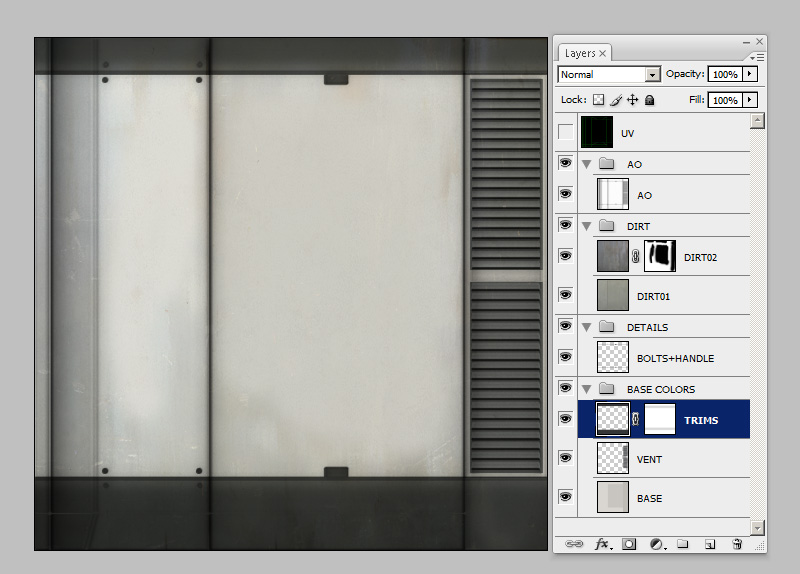
\includegraphics[width=0.415\linewidth]{bilder/vertexColorNoColor}\label{vertexColorNoColor}}%
  \qquad
  \subfloat[][Assets unter dem Einfluss Vertex Farben.]{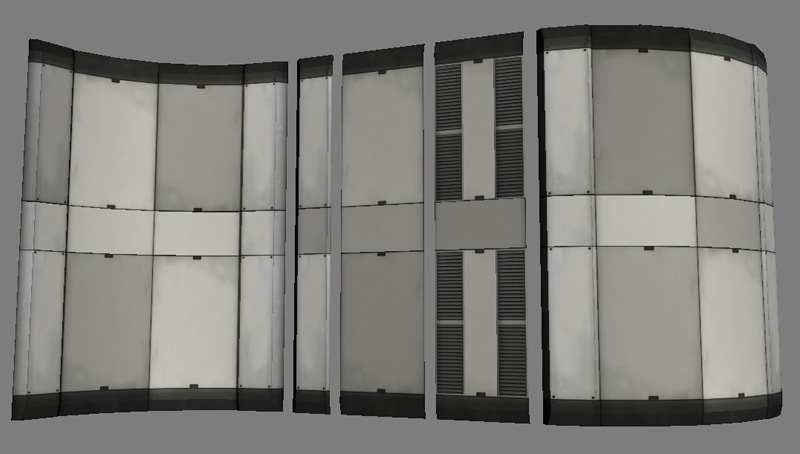
\includegraphics[width=0.525\linewidth]{bilder/vertexColor}\label{vertexColor}}%
  \caption{Beispiele für Einfluss von Vertex Farben \parencite{Klevestav}.}%
\end{figure}
\vspace{-10.5pt}
In 3D-Tools kann Vertices eines Meshes ein Farbwert zugeordnet werden. Diese Farbwerte heißen Vertex-Farben. Durch diese Technik kann, ohne großen Aufwand und ohne neue Objekte eine größere Anzahl Modelle erzeugt werden. In den Material-Einstellungen des Objekts muss angegeben werden, dass für die Farbgebung des Models die Vertex-Farben einkalkuliert werden sollen. Die Abbildungen \ref{vertexColorNoColor} \and \ref{vertexColor} zeigen, wie sich diese auf das Aussehen einer Textur auswirken können. \parencite{Klafke,Klevestav}
\subsection{Texturierung  von modularen Assets}
In dieser Thesis liegt der Fokus auf der Arbeit an den Modellen. Texturierung wird demzufolge nur angeschnitten.
\par
\begin{figure}[H]
\centering
  \makebox[\textwidth]{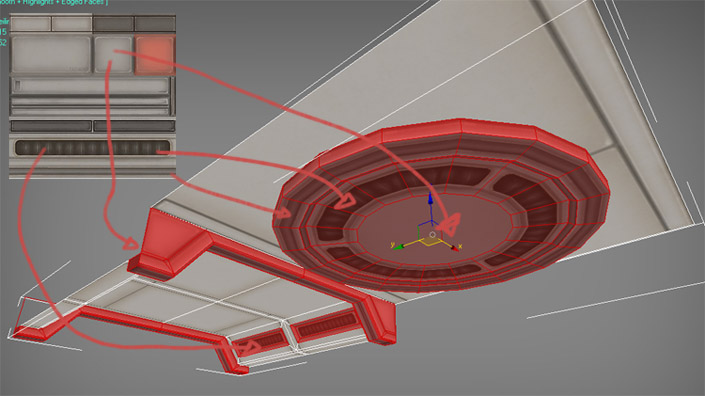
\includegraphics[width=0.72\linewidth]{bilder/trims}}
  \caption{Beispiel für Mehrfachnutzung eines Trimsheets \parencite{Klafke}.}
	\label{trims}
\end{figure}
\vspace{-10.5pt}
Modulare Elemente können wie normale Assets texturiert werden. Texturen von gemeinsam genutzten Objekten sollten aus Performance-Gründen auf einem Textur-Atlas verbunden werden. Nutzt ein Projekt Elemente, die mehrfach aneinandergefügt werden sollen, bietet es sich an, kachelbare Texturen zu nutzen. Auf diese Weise können große Flächen erzeugt werden, ohne Kanten oder sichtbare Nähte. Dies ist für modulare Assets von großem Vorteil. Da sie vielseitig nutzbar sind und nur einmal geladen werden müssen, sparen solche Texturen außerdem Ressourcen. \parencite{Meler}
\par
\begin{figure}[H]
\centering
  \makebox[\textwidth]{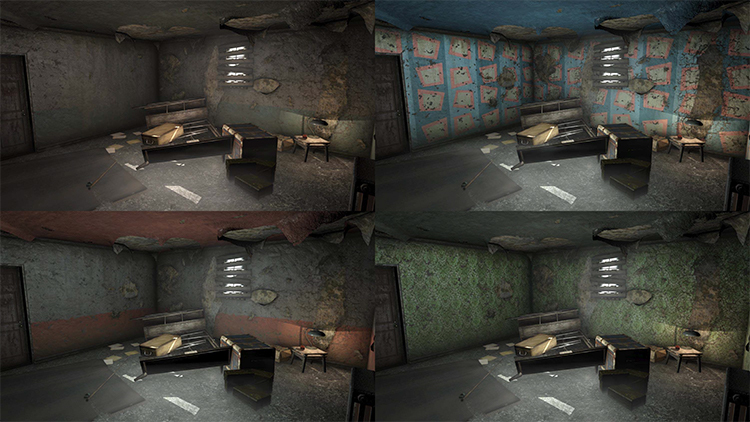
\includegraphics[width=0.72\linewidth]{bilder/MaterialSwap}}
  \caption{Ein Beispiel für das Potential austauschbarer Texturen. In Anlehnung an \parencite{Fallout4P}.}
	\label{MaterialSwap}
\end{figure}
\vspace{-10.5pt}
Werden austauschbare Texturen genutzt, die dem gleichen Aufbau folgen, kann ein Modell unterschiedlich aussehen. \parencite{Norris}
\par
Hiermit sind die Grundlagen für die praktische Ausarbeitung dieser Thesis abgeschlossen. Die nachfolgenden Kapitel wenden diese in der eigenen Umsetzung modularer Assets an.
\enlargethispage{11.5pt}